% TO-DO:
% * add decision surface 3D plot from Sage

\documentclass[orivec]{llncs}
\usepackage{graphicx}
\usepackage{amsmath}			% for "cases"
\usepackage{amsfonts}			% for frakur fonts
\usepackage{mathrsfs}			% for curly "E" error symbol
\usepackage{float}
\usepackage[most]{tcolorbox}	% for wrapping example in color box
% \usepackage{wrapfig}		% wrap figure beside text, used in example
\usepackage{tikz-cd}			% commutative diagrams
\usepackage{tikz}
\usepackage{amssymb}			% for \multimap \updownarrow \bigstar \varnothing
\usepackage{sectsty}			% change section color
% \usepackage{turnstile}		% longer turnstiles
\usepackage{wasysym}			% smileys
\usepackage[normalem]{ulem}	% underline with line breaks: /uline
\usepackage{hyperref}			% refs, links become clickable
\usepackage[]{algorithm2e}		% algorithms
%\usepackage[3D]{movie15}	% for embedding 3D shapes
%\usepackage[UKenglish]{babel}	% for movies or 3D
%\usepackage{media9}			% *** doesn't work

\usepackage{geometry}		% change paper size
\geometry{
  a4paper,         % or letterpaper
  textwidth=18cm,  % llncs has 12.2cm
  textheight=27cm, % llncs has 19.3cm
  heightrounded,   % integer number of lines
  hratio=1:1,      % horizontally centered
  vratio=2:3,      % not vertically centered
}
\usepackage[fontsize=13pt]{scrextend}

% *************** Delete when not using Chinese or colors **********************
\ifdefined\chinchin
\usepackage{xeCJK}
\setCJKmainfont[BoldFont=SimHei,ItalicFont=KaiTi]{SimHei}
\newcommand{\cc}[2]{#1}
\else
\newcommand{\cc}[2]{#2}
\fi

\usepackage{color}
\definecolor{cerulean}{RGB}{100,100,200}
\definecolor{darkgreen}{RGB}{10,130,10}
%\newcommand{\emp}[1]{\emp{\textcolor{Cerulean}{#1}}}
\newcommand{\emp}[1]{{\color{blue}\textbf{#1}}}
\definecolor{grey}{rgb}{0.98,0.98,0.98}
\definecolor{lightyellow}{rgb}{0.98,0.98,0.90}

% \chapterfont{\color{blue}}		% sets colour of chapters
\sectionfont{\color{blue}} 
\subsectionfont{\color{blue}} 
\subsubsectionfont{\color{blue}} 
\setcounter{secnumdepth}{3}		% use numbers in subsubsections
% \renewcommand\thesection{}		% hide section numbers (has bad indent effect)
% let\emptyset\varnothing			% more beautiful empty set symbol
\newcommand{\vect}[1]{\boldsymbol{#1}}
\newcommand*\sigmoid{\raisebox{-.2\height}{\includegraphics{sigmoid.png}}}
\newcommand*\stepfunction{\vcenter{\hbox{\includegraphics{step-function.png}}}}
\newcommand*\KB{\vcenter{\hbox{\includegraphics{KB-symbol.png}}}}
\newcommand*\NN{\vcenter{\hbox{\includegraphics{NN-symbol.png}}}}
\newcommand*\invsigmoid{\vcenter{\hbox{\includegraphics{inverse-sigmoid.png}}}}
\newcommand{\invW}{\, \rotatebox[origin=c]{90}{W}}
\newcommand{\invw}{\, \rotatebox[origin=c]{90}{w}}
\newcommand*\rectifier{\vcenter{\hbox{\includegraphics{rectifier.png}}}}
\newcommand{\dashh}{\textemdash~}
\newcommand{\tab}{\hspace*{1cm}}

\newcommand{\tikzmark}[1]{\tikz[overlay,remember picture] \node (#1) {};}

\let\labelitemi\labelitemii

\renewcommand{\thefootnote}{\fnsymbol{footnote}}
\interfootnotelinepenalty=10000

% ***** Boxed variables inside math equations
% \newcommand*{\boxedcolor}{black}
\makeatletter
% \renewcommand{\boxed}[1]{\textcolor{\boxedcolor}{%
% \fbox{\normalcolor\m@th$\displaystyle#1$}}}
% \setlength{\fboxsep}{1pt}
\renewcommand{\boxed}[1]{\fbox{\m@th$\displaystyle\scalebox{0.9}{#1}$} \,}
\makeatother

\overfullrule=0mm

\newsavebox{\MyName}
\savebox{\MyName}{\includegraphics[scale=0.6]{YKY.png}}


\cc{
\title{什么是神经网络?\\
	{\normalsize(中学数学程度可懂)}}
}{
\title{What are neural networks?\\
	{\normalsize (requires only high-school maths)}}
}
\titlerunning{\cc{什么是神经网络?}{What are neural networks?}}
\author{\usebox{\MyName} (King-Yin Yan)
% \\ \footnotesize{General.Intelligence@Gmail.com}
}
\institute{General.Intelligence@Gmail.com}

\begin{document}

\maketitle
\setlength{\parindent}{0em}
% \setlength{\parskip}{2.8ex plus0.8ex minus0.8ex}
\setlength{\parskip}{2.8ex}

%\begin{abstract}
%\end{abstract}

\cc{
人工智能中最重要的 3 大技术是:
\begin{itemize}
 \item 逻辑
 \item 神经网络
 \item 进化
\end{itemize}
神经网络属於统计学习 (statistical learning) 的一种,这些方法将 vector space 中的某些「点」分类。

Deep learning 的意思,简单来说,是「\emp{很多层}的神经网络」。 深度学习是目前人工智能中最备受瞩目的一种技巧。
}{
The 3 main approaches in artificial intelligence are:
\begin{itemize}
	\item logic
	\item neural networks
	\item evolution
\end{itemize}
Neural networks is a special kind of \textbf{statistical learning}, that operates on ``points'' in a vector space.

Deep learning is the hottest technique in current AI research.  ``Deep'' simply means ``many layers of neural networks''.
}

\section*{\cc{生物的神经细胞}{Biological neurons}}

\cc{
温习一下在中学时学过的生物学 {\Large \smiley}
}{
Let's refresh some high-school biology {\Large \smiley}
}

\cc{
这是一粒真的神经元:
}{
This is a biological neuron:
}
\begin{equation}
\vcenter{\hbox{\includegraphics[scale=0.4]{neuron.png}}}
\end{equation}
\cc{
细胞周围的 dendrites \emp{收集}电信号,当这些脉冲信号的\emp{总和}超过某一阀值 (threshold) 时,会\emp{发射} (fire) 一个电脉冲信号,从 axon 输出到另一神经元:
}{
Dendrites \textbf{collect} electrical signals;  When the \textbf{total} of these signals exceed a certain \textbf{threshold}, the neuron \textbf{fires} an electric impulse, sending to another neuron via the \textbf{axon}:
}

\begin{equation}
\vcenter{\hbox{\includegraphics[scale=0.5]{neuron-firing.png}}}
\end{equation}
\cc{
数学上我们将这过程极度简化,变成这样的模型 (model):
}{
Mathematically, this can be greatly simplified to such a \textbf{model}:
}
\begin{equation}
\vcenter{\hbox{\includegraphics[scale=0.75]{neuron-model.png}}}
\end{equation}
\cc{
意思是: 将每个输入加权 (weighted) 加起来,然后经过一个 $\sigmoid$ 形状的函数输出。 
}{
That means:  each input value is \textbf{weighted} and then summed together, and then passes through a $\sigmoid$ function for output.
}

\cc{
用数式表示:
}{
In formula:
}
\begin{equation}
\boxed{output} \; y = \sigmoid \; [ \; \sum_i (w_i \; x_i) \; ]
\end{equation}
\cc{
其中 $\sigmoid$ = sigmoid 函数是:
}{
where $\sigmoid$ = sigmoid function, is defined by:
}
\begin{equation}
\sigmoid (x) = \frac{1}{1 + e^{-x}}
\end{equation}
\cc{
它的形状是这样的:
}{
Its shape is like this:
}
\begin{equation}
\vcenter{\hbox{\includegraphics[scale=0.55]{sigmoid-graph.png}}}
\end{equation}
\cc{
它代表在左边没有信号 (0 = nothing),在右边的信号值是 1 = ``yes''。
}{
On the left it is 0 = nothing (no signals), on the right it is 1 = ``yes''.
}

\cc{
其实也可以用以下这些函数模拟 threshold 的作用:
}{
These functions are also feasible candidates for the ``threshold'':
}
\begin{equation}
\vcenter{\hbox{\includegraphics[scale=0.5]{../agi-17/activation-functions.png}}}
\end{equation}

\begin{tcolorbox}[colback=lightyellow, breakable, enhanced]
\emp{Fun fact \#1}\\

\cc{
神经细胞的表面布满了 sodium-potassium (Na$^+$/K$^+$) channels,它们用 ATP (adenosine triphosphate, 细胞的能量来源)以 3 Na$^+$ : 2 K$^+$ 的比例将 ions「泵」到细胞内,造成电压差。 这些蓄势待发的电压,当电压超过 threshold 时某些 channels 打开,造成 ``action potential''。 这个现象可以用微分方程描述,即著名的 Hodgkin-Huxley 方程,及其简化版本 FitzHugh-Nagumo 方程。\\

这 action potential 最特别的地方是: 它是一个 \emp{all-or-nothing} effect,亦即是说,如果输入总和低於阀值,则输出信号是平的 (zero)。 为什么要这样呢?  因为人的脑袋是由一些水母那样的\emp{多细胞}生物进化出来的,这些细胞之间慢慢学会用电信号 communicate,但它们在一滩水那样的环境下通讯,\emp{噪音}很大。 直到现在人脑仍然是像一碗汤水那样的环境,而且人要活动,脑部不停有微小震动,造成\emp{heat noise}。 为了要在噪音中运作,必须有机制将噪音\emp{抑制}下去,这就是 all-or-nothing 的原因。 换句话说,人脑的意识,其资讯是\emp{有限}的,就像电脑一样,并没有什么神秘。
}{
The surface of the neuron is covered with sodium-potassium (Na$^+$/K$^+$) channels, that use ATP (adenosine triphosphate, the energy source in the cell) to ``pump'' ions into the cell with a 3 Na$^+$ : 2 K$^+$ ratio, creating a voltage difference.   When the voltage exceeds the threshold, certain ion channels open, the built-up voltage is released to create an ``action potential''.  This phenomenon can be described using differential equations, that is the famous \textbf{Hodgkin-Huxley} equation, and its simplified version, the \textbf{FitzHugh-Nagumo} equation.\\

A very special feature about the action potential is that it is ``\textbf{all-or-nothing}'', ie, if the input is below threshold, the output signal would be flat (zero).  Why is it like this?  That is because the human brain evolved from primitive \textbf{multi-cellular} organisms (like the jellyfish) whose cells gradually learned to use electric signals to communicate.  They operated in an environment like a pool of water, in which there is a lot of \textbf{noise}.  Even now the human brain is like a pool of liquid, and the body is in constant motion, resulting in \textbf{heat noise}.  In order to operate within such noise, there must be a mechanism to \textbf{suppress} the noise;  This is the reason for all-or-nothing.  That is to say, human consciousness has \textbf{finite} information content, similar to a digital computer, and is not mysterious.
}
\end{tcolorbox}

\begin{tcolorbox}[colback=lightyellow, breakable, enhanced]
\emp{Fun fact \#2} \\

\cc{
神经细胞的\emp{细胞膜}是由 lipid bi-layer 构成,它的成份是脂肪和胆固醇 (cholesterol)。 胆固醇的作用是稳固细胞膜结构,每粒细胞都需要胆固醇。 脑里面的神经线全都是用细胞膜组成,所以脑基本上都是脂肪和胆固醇。  尤其是中国人吃的猪脑,它的胆固醇含量是所有食物中最高的,高出鸡蛋很多倍! \\

那层 myelin sheath 是脊椎类动物才有的,它好像电线外面的胶套,作用是加快神经传播的速度。 八爪鱼是无脊椎动物,所以它的头很大,牠比其他同类聪明,但脊椎类动物的脑袋可以较细小也达到同样的智力水平。
}{
The neuron's \textbf{cell membrane} is a \textbf{lipid bi-layer}, made up of fats and cholesterol.  The function of cholesterol is to make the membrane structurally stable, therefore every cell needs cholesterol.  The ``wires'' in the brain are all made of cell membranes, so the brain is basically made up of fats and cholesterol.  In particular, the pig's brain which is a kind of Chinese food, has the highest cholesterol content of all foods, many times more than eggs! \\

The \textbf{myelin sheath}, unique to vertebrates, is like the plastic insulation of electric wires, whose effect is to speed up electrical transmission.  The octopus is an invertebrate, that's why it needs a big head to achieve the same level intelligence as vertebrate animals of comparable brain size.
}
\end{tcolorbox}

\begin{tcolorbox}[colback=lightyellow, breakable, enhanced]
\emp{Fun fact \#3} \\

\cc{
神经信号传递到末梢 (synapse),不再用电传递,而是用化学分子 neuro-transmitter。 这些分子种类很多,例如抗抑郁药物常常提到的 serotonin 和 dopamine。 但其实最常见的 neurotransmitter 是 glutamate,它是所有动物的神经系统的主要通讯分子。 植物没有神经系统,所以植物里面没有 glutamate。 人类喜欢吃肉,所以进化出对肉类的味觉,特别喜欢 glutamate 的味道。 有个日本科学家发现了海藻内有一种物质,加进食物中可以做到肉的鲜味效果。  其实这种物质就是 glutamate,也就是「味精」。 所以味精其实对人体没有害,只是经常吃味精而不吃真的肉,会导致营养不均衡。 
}{
When the nerve signal reaches the \textbf{synapse}, it no longer uses electrical transmission, but switches to chemical transmission with \textbf{neuro-transmitter} molecules.  There are many types of neuro-transmitters, such as \textbf{serotonin} and \textbf{dopamine}, often mentioned in anti-depression drugs.  But the most common neuro-transmitter is \textbf{glutamate}, the main signaling molecule for the nervous systems of all animals.  Plants lack a nervous system, therefore glutamate is not found in plants.  Humans like to eat meat, so we evolved a taste for meat, especially the taste for glutamate.  A Japanese scientist discovered a substance in sea-weed, which when added to food mimics the taste of meat.  Actually this substance is just glutamate, or MSG (mono-sodium glutamate).  So MSG is not harmful to humans, it's just that we may not get a balanced nutrition if we eat MSG often instead of real meat.
}
\end{tcolorbox}

\section*{\cc{一粒神经元的几何解释}{1 neuron -- geometric interpretation}}

\cc{
以前说过,\emp{机器学习}的目标通常是将空间上的某些「点」\emp{分类}:
}{
As I explained in other tutorials, the goal of \textbf{machine learning} is usually to \textbf{classify} certain ``points'' in a space:
}
\begin{equation}
\vcenter{\hbox{\includegraphics[scale=0.6]{ML-example.png}}}
\end{equation}

\cc{
例如,在\emp{机器视觉}中,一张图像可以有几万个 pixels,每个 pixel 是一个\emp{维度},它的\emp{颜色}就是这个维度上的\emp{座标值}。 整个空间就是\emp{所有图像}的空间,\emp{每一点}是一个图像,这种空间的维数很高(维数就是一张图像的 pixels 个数)。 通常我们讲解时用 2 维或 3 维空间,读者们要运用想像力幻想一下很高维的情况。
}{
For example, in \textbf{machine vision}, a picture can have millions of \textbf{pixels}, each pixel being a dimension, its \textbf{color} is the \textbf{coordinate value} on this dimension.  The entire space is the space of \textbf{all images}, with each \textbf{point} representing an image.  The dimensionality of such spaces is very high (the dimension is the number of pixels per image).  We often use 2 or 3 dimensions for explaining things, but the reader should use their imagination for higher dimensions.
}

\cc{
在中学数学中有学过,一条\emp{直线}的方程是这形式的:
}{
We know from high-school maths, the equation for a \textbf{straight line} is:
}
\begin{eqnarray}
& \mbox{\footnotesize \color{red}{constants}} \tikzmark{constants} \nonumber \\
\nonumber \\
& {\color{red}{a}} \tikzmark{constA} x \tikzmark{varX} + {\color{red}{b}} \tikzmark{constB} y \tikzmark{varY} + {\color{red}{c}} \tikzmark{constC} = 0 \\
\nonumber \\
& \mbox{\footnotesize variables} \tikzmark{variables} \nonumber
\begin{tikzpicture}[overlay,remember picture]
  \draw[red] (constants.center) +(-30pt,-4pt) -- ([shift={(-3pt,8pt)}]constA.center);
  \draw[red] (constants.center) +(-20pt,-4pt) -- ([shift={(-1pt,10pt)}]constB.center);
  \draw[red] (constants.center) +(-10pt,-4pt) -- ([shift={(-1pt,8pt)}]constC.center);
  \draw (variables.center) +(-29pt,8pt) -- ([shift={(-4pt,-2pt)}]varX.center);
  \draw (variables.center) +(-15pt,8pt) -- ([shift={(-4pt,-4pt)}]varY.center);
\end{tikzpicture}
\end{eqnarray}

\cc{
它的\emp{几何}解释是这样的:
}{
Its \textbf{geometric interpretation} is like this:
}
\begin{equation}
\vcenter{\hbox{\includegraphics[scale=0.75]{linear-inequality.png}}}
\end{equation}
\cc{
在直线上,那直线的方程 $= 0$。 直线将它身在的空间\emp{分割}成两半: 一边 $> 0$,另一边 $< 0$。
}{
For points on the line, the equation is $= 0$.  The line \textbf{cuts} the space into 2 halves:  one side is $> 0$, the other $< 0$.
}

\cc{
推广到 3 维空间的情况,我们有一个\emp{平面}的方程: 
}{
Generalizing to 3-dimensions, we have the equation for a \textbf{plane}:
}
\begin{equation}
{\color{red}{a}}x + {\color{red}{b}}y + {\color{red}{c}}z + {\color{red}{d}} = 0
\end{equation}
\cc{
它同样将空间\emp{分割}成两半,一半 $> 0$,另一半 $< 0$:
}{
It also \textbf{cuts} the space into 2 halves, one side $> 0$, the other $< 0$:
}
\begin{equation}
\vcenter{\hbox{\includegraphics[scale=0.75]{linear-inequality-2.png}}}
\end{equation}

\cc{
在任意 $n$-维空间,每一点记作 $\vect{x} = (x_1, x_2, ..., x_n)$,一个\emp{超平面} (hyper-plane) 将该空间分割成两半,它的方程是: 
}{
For arbitrary $n$-dimensions, with each point denoted as $\vect{x} = (x_1, x_2, ..., x_n)$, a \textbf{hyperplane} cuts the space into 2 halves, its equation is:
}
\begin{equation}
{\color{red}{a_1}}x_1 + {\color{red}{a_2}}x_2 + .... + {\color{red}{a_n}}x_n + {\color{red}{a_0}} = 0
\label{eqn:general-linear}
\end{equation}

\begin{tcolorbox}[colback=lightyellow, breakable, enhanced]
\cc{
注意: 一块超平面的维数是多少? 在平面空间里它是一条线(1 度空间),在立体空间里它是平面(2 度空间), 一般来说,在 $n$-维空间里的超平面是一个 $n - 1$ 维的物体,$(n-1)$ 又叫作 co-dimension 1,意思是说 ambient space 的维数是 $n$,方程 (\ref{eqn:general-linear}) 减少了一个\emp{自由度} (degree of freedom),所以\emp{服从}这等式的物体内,只有 $n - 1$ 个自由度。 
}{
Note:  What is the dimension of a hyper-plane?  In 2-D space, it is a line (1-D), in 3-D space, it is a plane (2-D);  In general, in $n$-D space a hyper-plane is an $(n - 1)$-dimension object, $(n-1)$ is also called \textbf{co-dimension 1}, meaning that the ambient space is of dimension $n$, and equation (\ref{eqn:general-linear}) reduces the \textbf{degrees of freedom} by 1, so the object \textbf{constrained} by this equation has $n - 1$ degrees of freedom.
}
\end{tcolorbox}

\cc{
现在可以看到超平面和神经元之间有些相似,因为神经元在未经过 $\sigmoid$ 之前,就是一个 \emp{线性组合}: 
}{
Now we can see some resemblance between the hyper-plane and the neuron, as the neuron is a \textbf{linear combination} before passing to the $\sigmoid$:
}
\begin{eqnarray}
& \mbox{\footnotesize \color{red}{linear combination}} \nonumber \\
\boxed{output} \; y = \sigmoid & [ \; \overbrace{\sum_i (w_i \; x_i)} \; ]
\end{eqnarray}
\cc{
换句话说: \uline{每粒神经元构成一超平面,它将空间切割成两半}。
}{
That is to say:  \uline{Each neuron forms a hyper-plane, that cuts the space into 2 halves}.
}

\cc{
加了 $\sigmoid$ 之后怎样? 未有 $\sigmoid$ 时,分割的两边分别是 $> 0$ 和 $< 0$,如果将颜色看作是「强度」,强度是逐渐变化的:  (右边表示从侧面看,立体)
}{
What if $\sigmoid$ is applied?  Without $\sigmoid$, the 2 halves are $> 0$ and $< 0$;  Now if we see colors as ``intensity'', the intensity changes gradually:  (the figure on the right shows the side view, as in 3-D)
}
\begin{equation}
\vcenter{\hbox{\includegraphics[scale=0.6]{linear-inequality-3.png}}}
\end{equation}
\cc{
加了 sigmoid 之后,用 1 代表「yes」,0 代表「no」,则两边的对比加强了,亦即更\emp{两极化}、「非此即彼」:
}{
When $\sigmoid$ is applied, 1 represents ``yes'' and 0 represents ``no'', so the contrast between the 2 sides is enhanced, ie, more \textbf{polarized}, or binary:
}
\begin{equation}
\vcenter{\hbox{\includegraphics[scale=0.6]{linear-inequality-4.png}}}
\end{equation}

\section*{\cc{> 1 粒神经元}{$> 1$ neurons}}

\cc{
如果有 $> 1$ 粒神经元(在同一层上),例如 3 粒:
}{
If there are $> 1$ neurons (on the same layer), eg. 3:
}
\begin{equation}
\vcenter{\hbox{\includegraphics[scale=0.6]{linear-inequalities-1.png}}}
\label{simple-network-layer}
\end{equation}
\cc{
注意: 座标是 $(x_1, x_2) = $ 输入,输出是 $(y_1, y_2, y_3)$,分别用 3 条{\color{red}{虚线}}代表。 这\emp{一层}神经网络的 network topology 如 (\ref{simple-network-layer}) 右图所示(每粒神经元没有画出 $\sum$ 和 $\sigmoid$)。
}{
Note:  The coordinates are $(x_1, x_2) = $ input.  Output is $(y_1, y_2, y_3)$, represented by 3 {\color{red}{dotted}} lines.  The \textbf{network topology} of this \textbf{1 layer} of neural network is as shown on the right (The $\sum$ and $\sigmoid$ for each neuron are not shown).
}

\cc{
每粒神经元可以选择某一边为「yes」,这些选择的 conjunction 可以形成不同的形状,例如以下两种: 
}{
Each neuron may choose one side to be ``yes''.  The \textbf{conjunctions} of these choices may form various shapes, eg:
}
\begin{equation}
\vcenter{\hbox{\includegraphics[scale=0.6]{linear-inequalities-2.png}}}
\end{equation}
\cc{
亦注意在右图中,可以出现几个 disjoint regions(在空间上分离的)。
}{
Also notice that in the right figure, a number of disjoint regions (separated in space) are possible.
}

\cc{
很明显,可以用神经元将输入空间的点进行切割和分类,达到\emp{机器学习}的目的。
}{
Obviously, we could use neurons to separate and classify points in space, thus achieving the goal of \textbf{machine learning}.
}

\section*{\cc{一层神经网络}{1 layer of neurons}}

%简单来说,当神经网络的\emp{层数}增加,在输入空间的切割形状会变得更为\emp{复杂},所以多层的神经网络有能力学习出非常复杂的 patterns,这就是\emp{深度学习}的优势。

\cc{
接下来要用到更多 \emp{线性代数},我会在另一篇 tutorial 解释。 
}{
In this part we need more \textbf{linear algebra}, which I will explain in another tutorial.
}

\cc{
一层神经网络的数学形式是:
}{
The mathematical form of 1 layer of neural network is:
}
\begin{equation}
\boxed{output} \; \vect{y} = \sigmoid [ W \vect{x} ] 
\end{equation}
\cc{
其中 $W$ 是矩阵,亦即 \emp{线性变换}; $\sigmoid$ 是 \emp{非线性变换}。
}{
where $W$ is a matrix, ie. a \textbf{linear transformation}; $\sigmoid$ is a \textbf{non-linear transformation}.
}

\cc{
矩阵是 \emp{线性方程组} 的紧凑写法。 一粒神经元 = $\sigmoid \circ \boxed{线性组合}$,一条线性组合是矩阵中的一行。
}{
Matrices are a compact way of writing \textbf{systems of linear equations}.  1 neuron = $\sigmoid \circ \boxed{linear combination}$, each linear combination is a \textbf{row} in a matrix.
}

\cc{
每一个矩阵都代表一个 \emp{linear transformation}:
}{
Every matrix is a representation for a \textbf{linear transformation}:
}
\begin{equation}
\vcenter{\hbox{\includegraphics[scale=0.6]{linear-transformation.png}}}
\end{equation}
\cc{
线性变换可以将正方形「扯」成平行四边形,也包括位置上的\emp{旋转} (rotation) 和\emp{平移} (translation)。 但直线仍变为直线,故名。
}{
Linear transformations can ``skew'' a square into a parallelogram, and also include \textbf{rotations} and \textbf{translations}.  Straight lines are preserved as straight lines, hence its name.
}

\cc{
另外要明白 $\sigmoid$ 变换的形状: (以下是 $x$ 和 $y$ 座标都被 sigmoid 变换)
}{
Next we need to know what $\sigmoid$ does:  (below is the sigmoid transform of both $x$ and $y$ coordinates)
}
\begin{equation}
\vcenter{\hbox{\includegraphics[scale=0.75]{sigmoid-transforms.png}}}
\end{equation}
\cc{
可以这样理解 $\sigmoid$: 它将平面上的点「扯向」4个角位,,所以我变了「国字口面」。
}{
$\sigmoid$ can be seen as ``stretching'' the square to its 4 corners, so I take on the ``square-face'' look.
}

\cc{
我们说这些顶点是\emp{吸引子} (attractors):
}{
We say that these vertices are \textbf{attractors}:
}
\begin{equation}
\vcenter{\hbox{\includegraphics[scale=0.75]{attractors.png}}}
\end{equation}

\cc{
注意: 在 $\sigmoid$ 变换时,图像是从周围\emp{无限}的空间压缩到 $[-1,+1]^2$ 这方格里:
}{
Note:  During the $\sigmoid$ transform, the image is compressed from the \textbf{infinite} unbounded space to the $[-1,+1]^2$ square:
}
\begin{equation}
\vcenter{\hbox{\includegraphics[scale=0.6]{sigmoid-transform-1.png}}}
\end{equation}

\cc{
以下是\emp{一层}神经网络的变换,分解成 $W$ 和 $\sigmoid$ 两部分:
}{
Here is the transformation performed by \textbf{1 layer} of neural network, decomposed into the $W$ and $\sigmoid$ parts:
}
\begin{equation}
\vcenter{\hbox{\includegraphics[scale=0.6]{NN-1-layer.png}}}
\end{equation}

\begin{tcolorbox}[colback=lightyellow, breakable, enhanced]
\section*{\cc{Sigmoid distortion 程式}{Code for sigmoid distortion}}

\cc{
这个 Python 程式没有用到图像处理的 sampling 技巧,纯粹是简单的示範。 改编自 Prateek Joshi 的《\textit{OpenCV with Python by example}》的 image warping 例子: \\  % 需要 install OpenCV 2 和 NumPy。
}{
This Python program is adapted from Prateek Joshi's $\langle$\textit{OpenCV with Python by example}$\rangle$, section on ``image warping''.  It is just a simple demo, which does not use advanced image sampling techniques. \\
}
\footnotesize \url{https://www.packtpub.com/mapt/book/application_development/9781785283932}

\footnotesize
\begin{verbatim}
import cv2
import numpy as np
import math

img = cv2.imread("input.jpg", cv2.IMREAD_GRAYSCALE)
Y, X = img.shape                     # size of the image
print "X = ", X
print "Y = ", Y

img_out = np.zeros(img.shape, dtype=img.dtype)

k = 80.0                             # scaling factor (smaller = more distorted)

for y in range(Y):
    outsideX = False                 # out-of-boundary
    y0 = Y / (y + 0.5)               # y-position in original image scaled to [0,1]
    y1 = -k * math.log(y0 - 1.0)     # new position
    y2 = int(y1 + Y/2.0)             # adjust for mid-point
    if y2 >= Y or y2 < 0:            # out of boundary?
        outsideX = True
    for x in range(X):
        outsideY = False
        x0 = X / (x + 0.5)
        x1 = -k * math.log(x0 - 1.0)
        x2 = int(x1 + X/2.0)
        if x2 >= X or x2 < 0:
            outsideY = True
        if not (outsideX or outsideY):
            img_out[y,x] = img[y2,x2]
        else:
            img_out[y,x] = 255       # white color if out-of-bounds

cv2.imshow("Input", img)
cv2.imshow("Distorted", img_out)
cv2.imwrite("output.jpg", img_out)
\end{verbatim}
\normalsize

\cc{
有兴趣的读者可以写一个游戏,「手动」地旋转 $W$ 矩阵,在 3D 或 4D 投影中分辨一些 patterns。
}{
The interested reader can try to make a game, where the player manually ``rotate'' the $W$ matrix of a neural network, to recognize some visual patterns (perhaps projected from 3D or 4D to 2D).
}
\end{tcolorbox}

%为简化讨论,现在只考虑 2 粒神经元的\emp{输入}和\emp{输出}空间(都是 2 度空间的平面):
%\begin{equation}
%\vcenter{\hbox{\includegraphics[scale=0.6]{linear-inequalities-3.png}}}
%\end{equation}
%因为 $\sigmoid$ 的缘故,输出的位置会趋近 hyper-cube 的那些 \emp{顶点} ({\color{red}{\textbullet}})。 这些顶点对应於输入空间中被割开的 regions。 例如 {\color{cerulean}{蓝色}}那块 region 对应於:
%\begin{equation}
%(y_1 = \mbox{yes}, y_2 = \mbox{yes}) \quad \Rightarrow \quad (1,1)
%\end{equation}
%当输入位置随{\color{darkgreen}{绿色}}线游荡时,输出会在 hyper-cube 的顶点之间跳来跳去。 妳可能觉得这样移动很无聊(因为顶点个数不多),但当神经元的个数 $n$ 增加时,hyper-cube 的顶点个数会以 $2^n$ 的速度增长。 

\section*{\cc{一层神经网络的 inverse}{The inverse of 1 layer}}

\cc{
现在再考虑,经过一层之后,如果在 target space 有一条 \emp{直线}(或者叫 linear discriminant),那么这条直线在 original space 会是什么形状?  这个形状就是 \emp{decision boundary},亦即是说,我们在 target 空间切了「线性的一刀」,在原空间这刀割的形状是怎样? 
}{
Now we consider the inverse of the 1-layer network:  if we have a \emp{straight line} (or ``linear discriminant'') in the target space, what would this line look like in the original space?  This is the so-called ``decision boundary'', that is to say, if we make a ``linear cut'' in the target space, what would be the shape of our ``knife'' in the original space?
}

\cc{
在 target 空间的线性分割是:
}{
A linear cut in the \textbf{target} space is:
}
\begin{equation}
a x' + b y' + c = 0
\end{equation}
\cc{
神经网络的变换是:
}{
The 1-layer neural network transforms it via:	
}
\begin{equation}
(x' \; y') = \sigmoid W \genfrac(){0pt}{0}{x}{y}
\end{equation}
\cc{
假设 $W = \mbox{id}$(忽略 $W$ 的作用),则变换简化成:
}{
Suppose $W = \mbox{id}$ (ignoring the effect of $W$), then the transform becomes:
}
\begin{equation}
\begin{cases}
x' = \sigmoid x \\
y' = \sigmoid y
\end{cases}
\end{equation}
\cc{
原空间的方程就是:
}{
The equation of the ``cut'' in the original space is thus:
}
\begin{equation}
\frac{a}{1 + e^{-x}} + \frac{b}{1 + e^{-y}} + c = 0
\end{equation}
\cc{
这家族的曲线(亦即是「刀的形状」)其中有些是这样的:
}{
This family of curves (ie, the ``shapes of the knifes'') are typically like these:
}
\begin{equation}
\vcenter{\hbox{\includegraphics[scale=0.6]{curves2.png}}}
\end{equation}
%\includemedia[
%  activate=onclick,
%  width=0.5\textwidth
%]{\includegraphics[scale=1.0]{movie.png}}{movie.flv}
\cc{
换句话说: 在 target 空间中的直线切割,在原空间中被「压向中心」,变成有一个弯位的曲线,这是 $\sigmoid^{-1}$ 的作用。
}{
In other words, linear cuts in the target space, got ``squeezed towards the center'' in the original space, which turns them into a curve with one bending, this is the effect of the $\sigmoid^{-1}$.
}

\begin{tcolorbox}[colback=lightyellow, breakable, enhanced]
\section*{\cc{Mathematica 程式}{Mathematica code}}

\footnotesize
\begin{verbatim}
Manipulate[
    GraphicsGrid[{{
        ContourPlot[a x + b y + c == 0, {x, -10, 10}, {y, -10, 10} ],
        ContourPlot[a/(1 + Exp[- k x]) + b/(1 + Exp[- k y]) + c == 0,
            {x, -10, 10}, {y, -10, 10} ]
        }}],
    {{a, .1}, -10, 10, .01},
    {{b, -.2}, -10, 10, .01},
    {{c, 0}, -10, 10, .05},
    {{k, 1}, 0.5, 5}]
\end{verbatim}
\normalsize

\cc{
读者可以在 Mathematica 试验这些曲线的形状: 左边是 target 空间的直线,右边是它在原空间的曲线:
}{
Readers can try out the shape of these curves in Mathematica.	On the left is the straight line in target space, on the right the curve in original space:
}
\begin{equation}
\vcenter{\hbox{\includegraphics[scale=0.75]{Mathematica-manipulate.png}}}
\end{equation}
\end{tcolorbox}

\cc{
注意,如果在 $\sigmoid$ 中加入参数 $\tau$ 变成:
}{
Notice:  if we add a $\tau$ parameter into the $\sigmoid$ function:
}
\begin{equation}
\sigmoid (x) = \frac{1}{1 + e^{-\tau x}}
\label{tau-time}
\end{equation}
\cc{
则当 $\tau \rightarrow \infty$ 时, $\sigmoid$ 变成 $\stepfunction$,而这些曲线也逐渐变成「角」的形状 \footnote{但其实当 $\tau \rightarrow \infty$ 时,在 target 空间只存在 4 个离散的顶点,所以那直线会变成 undefined。\\
在这篇文章的较早版本中,我错误地说,当 $\tau \rightarrow 0$ 时,$\sigmoid (x) \rightarrow f(x) \equiv x$; 其实 $\sigmoid$ 会变成一个常函数,即 $f(x) \equiv 1/2$。
}:
}{
When $\tau \rightarrow \infty$, $\sigmoid$ turns into $\stepfunction$, and these curves turn into ``corner'' shapes.  \footnote{Actually, when $\tau \rightarrow \infty$, the target space degenerates into 4 vertex points, and those straight lines become \textbf{undefined}. \\
In a previous version of this tutorial, I mistakenly claimed that $\sigmoid (x) \rightarrow f(x) \equiv x$ as $\tau \rightarrow 0$.  In fact $\sigmoid$ would become a constant function, $f(x) \equiv 1/2$ as $\tau \rightarrow 0$.}:
}
\begin{equation}
\vcenter{\hbox{\includegraphics[scale=0.6]{towards-angular.png}}}
\end{equation}
\cc{
这表示,在 $\tau \rightarrow \infty$ 时,decision boundary 会分割 4 个角位。 
}{
This shows that when $\tau \rightarrow \infty$, the decision boundary is divided into 4 corner positions.
}

\cc{
讲了这么多,最重要的 insight 似乎是:  \uline{每个神经元所 represent 的其实只是一个 \emp{binary feature}}。 
}{
So much for this, and the most important insight seems to be this:  \uline{Each neuron represents a binary feature}.
}

% ***************** Does not work in XeLatex ***************
%\includemovie[
%	poster,
%	toolbar,
%	label=angular.u3d,
%	text=(angular.u3d),
%	3Daac=60.000000, 3Droll=0.000000, 3Dc2c=0.006653 -34.630001 0.000000, 3Droo=34.630001, 3Dcoo=0.006653 0.000000 0.000000,
%	3Dlights=CAD,
%]{\linewidth}{\linewidth}{angular.u3d}

\section*{\cc{多层神经网络}{Multi-layer neural network}}

\cc{
多层只是单层的重复:
}{
Multi-layer is simply the repetition of single layers:
}
\begin{equation}
\boxed{output} \; \vect{y} = \sigmoid \stackrel{1}{W} \; \sigmoid \stackrel{2}{W} \; ..... \; \sigmoid \stackrel{L}{W} \; \vect{x}
\end{equation}
$L$ = total number of layers.

\cc{
「训练」神经网络的方法是通过著名的 \emp{反向传递} 算法,在很多教科书和网上文章中已有介绍,所以我不复述。  基本上,我们给定一对对的输入值和期望的输出值,而网络的输出值和期望值之间会有一些差距,此即为 ``error'',反向传递算法 的目的是要调教网络的 weights,使误差的总和达到最小值。  调教的方法是「梯度下降法」,这是最优化理论中最常见的一个算法。
}{
The way to ``train'' a neural network is by the famous \emp{back-propagation} algorithm, which I won't explain here because it is contained in many standard texts or online tutorials.  Basically, the network is given pairs of inputs and their desired outputs.  There will be a gap between the network's own output and the desired output, ie, the ``error''.  Back-prop tries to adjust the weights to minimize the total error.  It does this via \emp{gradient descent}, a standard optimization algorithm.
}

\cc{
在我想像中,多层神经网络的运作好像「拉面条」: (这只是示意图)
}{
In my mind, a multi-layer neural network acts like ``pulling and twisting a bunch of noodles'': (the diagram is meant to be illustrative only)
}
\begin{equation}
\vcenter{\hbox{\includegraphics[scale=0.75]{ramen-noodle-1.png}}}
\end{equation}
\cc{
如果将 $\sigmoid$ 函数扯成一直线,则这些「面条」会 ``unwind'' 成简单的一个线性变换:
}{
By deforming the $\sigmoid$ function to a straight line, the noodles can be ``unwinded'' to a simple linear transformation:
}
\begin{equation}
\vcenter{\hbox{\includegraphics[scale=0.75]{ramen-noodle-2.png}}}
\end{equation}
\cc{
% $\tau$ 可以看成是一个「另类时间」。 
暂时我不知道这个想法有什么应用; 或许和 braid theory 有关? 

也可以看出: 每个神经元的数值输出,其实没有 fuzzy value 的意义,而仅仅是带有某些 topological 信息而已(亦即哪些点和哪些点邻近)。 然而,神经网络可以近似任何函数,我们可以令它学习输出 fuzzy values,只要适当地设定 \emp{目标函数} 即可。 
}{
% where $\tau$ can be regarded as an ``alternative time''.
At this point I don't know what is the use of this observation, perhaps it could be related to \emp{braid theory}?

We also observe that the ouput of each neuron does not contain ``fuzzy value'' information, only \textit{topological} information (ie, which points are neighbors with which points).  However, because the neural network is a universal function approximator, we can force it to learn fuzzy values as outputs, if we set the objective function appropriately.
}

{\color{red}TO-DO}: 
\cc{
还有一件想做的事,是 plot 出多層神经網絡的 error surfaces。 记忆中好像看过这些 error surface 有「楼梯级」的形状,这可能解释为什么训练时 error 会有「骤然下降」的现象,而这可能不是 phase transition 现象,而纯粹是 error surface 固有的形状而已。
}{
Another thing I want to do is to plot the error surfaces of a multi-layer neural network.	From what I've read, these error surfaces seem to have a ``staircase-like'' appearance.  This may explain why during the training of an NN, the error sometimes remains flat, punctuated by \textit{abrupt drops}, which may not be due to the phenomenon of \textit{phase transition}, but is merely a characteristic of the error surface.
}

\section*{\cc{和 Bayesian network 比较}{Comparison with Bayesian networks}}

\cc{
以上是对 NN 的「几何解释」,但其实有个更简单直接的解释是: NN 实现的是 \emp{命题逻辑} 的一种简单形式,例如以下的 Bayesian network 也可以看成是 NN 的一粒神经元,每个 node 代表一个命题: 
}{
The above is a ``geometric interpretation'' of neural networks, but there is also a simpler and more direct interpretation:  NN as a realization of \emp{propositional logic}.  For example, the Bayesian network below can be regarded as a \textit{neuron} within a neural network;  Each node of the Bayesian network represents a proposition:
}
\begin{equation}
\vcenter{\hbox{\includegraphics[scale=0.6]{flat-Bayes-net.png}}}
\end{equation}

\cc{
但神经元的 $\sigmoid \sum$ 运算太简单,不足以计算概率的准确值。 举例来说,在 Bayesian network 中有 ``explaining away'' 的现象,例如以下的「遗书」如果存在,会令「自杀」的机率提升,但也令「他杀」的机率下降:
}{
But a single neuron's $\sigmoid \sum$ operation is too simple, insufficient for calculating probabilities correctly.  For example, Bayesian networks are capable of ``explaining away'', such as in the Bayesian network below, if ``suicide note'' is true, then the probability of ``suicide'' increases, and the probability of ``murder'' decreases:
}
\begin{equation}
\cc{
\vcenter{\hbox{\includegraphics[scale=0.6]{suicide-note.png}}}
}{
\vcenter{\hbox{\includegraphics[scale=0.6]{suicide-note-en.png}}}
}
\end{equation}
\cc{
换言之,在 Bayesian network 中概率的计算是有传递性的,它需要用到复杂的 \emp{belief propagation} 算法,这个算法复杂是因为它严格遵守概率论,但神经网络的简单性似乎难做到这效果。
}{
In other words, the probabilities in a Bayesian network are all connected with each other, 	they require the use of \emp{belief propagation} algorithms to calculate, which are rather complicated, as they must obey the rules of probability theory.  It seems difficult for neural networks to emulate these calculations in a simple manner.
}

% {\centering{\rule[0.5ex]{8cm}{1pt}}}

\section*{\cc{和 decision tree 比较}{Comparison with decision trees}}

% Decision tree 可不可以学习 features / representations?  有两种分析: 每个输入是一个 binary attribute; 或者每个 attribute 是一个 linear discriminant。  

\cc{
重温一下 decision tree 的经典例子:
}{
Let us recall a classic example of decision trees:
}

\begin{equation}
\vcenter{\hbox{\includegraphics[scale=0.6]{decision-tree-classic-example.jpg}}}
\end{equation}
\cc{
这是 training data:
}{
This is the training data:	
}

\begin{equation}
\vcenter{\hbox{\includegraphics[scale=0.6]{decision-tree-classic-example-2.jpg}}}
\end{equation}
\cc{
Decision tree 是根据 attribute-value pairs 来进行分类的。 为了较接近和神经网络比较,我假设这 decision tree 的每个 attribute 都是一个\emp{线性分割}:
}{
Decision trees classify things according to \textbf{attribute-value} pairs.  In order to compare them with neural networks, we assume that each decision tree attribute is a \emp{linear cut}:
}
\begin{equation}
\sum a_i x_i \stackrel{?}{>} 0
\end{equation}
\cc{
Decision tree 有个特点: 每次分割之后,分开的两边是\emp{独立}处理的,彼此不再相关 \footnote{在图 (\ref{decision-tree-cuts}) 中分割很多次其实没有多大意义,因为输出只有 4 个「角位」而已。 有意义的分割在高维空间才看得出来。}:
}{
Decision trees have a special property:  after each cut, the 2 halves are processed \emp{separately}, and they have nothing to do with each other subsequently \footnote{In diagram (\ref{decision-tree-cuts}), cutting the 2D plane many times is not very meaningful, because the output has only the 4 corner vertices.  The cuts would be more meaningful when visualized in higher-dimensional space}. 
}
\begin{equation}
\vcenter{\hbox{\includegraphics[scale=0.6]{decision-tree-cuts.png}}}
\label{decision-tree-cuts}
\end{equation}
\cc{
例如在最上层做了~ 男生/女生~ 的分割后,接下来女生的分割可能是「漂亮」、「身材好」这些属性,而男生那边则是「高大」、「英俊」等; 男生和女生的重要属性不同。 可以说决策树做的是 ``\emp{shallow cut}'',和神经网络的 ``\emp{deep cut}'' 不同。 
}{
For example, if the top branch made a cut for ``boy / girls'', then subsequent cuts for girls may be for ``pretty'' or ``nice figure'', whereas for boys may be ``tall'' and ``handsome''.  The cutting attributes for boys and for girls are different.  We could say that decision trees have ``shallow cuts'', which are different from the ``deep cuts'' of neural networks.
}

\cc{
观察多层 NN 的表达式:
}{
If we look at the expression for a multi-layer neural network:
}
\begin{equation}
\boxed{output} \; \vect{y} = \sigmoid \stackrel{1}{W} \; \sigmoid \stackrel{2}{W} \; ..... \; \sigmoid \stackrel{L}{W} \; \vect{x}
\end{equation}
\cc{
可以看到,每一层的「分类」结果,\emp{全部}送到下一层再作分类。 这和 decision tree 的情况很不同: 后者在建立 \emp{分支} (branching) 之后,对每个分支的分类是独立的,即所谓 greedy algorithm。 这凸显出神经网络是一种很特殊的分类器,它自底层到高层、每层之间有「千丝万缕」的关系,所以能做到 representation learning 或 features learning 的效果。
}{
we can see that, for each layer, the results of ``classification'' are all passed down to the next layer.  This is very different from what happens in decision trees:  after each ``\emp{branch}'' of the cut, the branches are processed separately, the essence of the so-called ``greedy algorithm''.  This neural networks are a very special type of classifiers, wherein the higher and lower layers are ``intertwined'' with many many inseparable connections.  This is the reason why neural networks are capable of \emp{representation learning} and \emp{features learning}.
}

\section*{\cc{和命题逻辑的关系}{Relation to propositional logic}}

\cc{
早在 AI 初期,「AI 之父」 John McCarthy 已经意识到 NN 只是一种简单的命题逻辑,他觉得这是严重的局限。 但注意:如果 NN 底层的神经元是 sub-symbolic 的话,它可以有「创造」新命题的能力,这就比经典命题逻辑的表达力强很多了。 
}{
Back in the early days of AI, the ``father of AI'' John McCarthy has already recognized that neural networks are essentially a mimic of simple propositional logic, and he thinks this is a severe limitation.  But note that:  if the lower layers of the neural network can represent \emp{sub-symbolic} features, then it has the ability to ``create'' new propositions, and this would be much more powerful and expressive than classical propositional logic.
}

\cc{
\centering{ --- 完 --- }
}{
\centering{ --- The end --- }
}

% \href{http://genifer.googlecode.com/files/Genifer - induction (30 July 2012).pdf}{inductive learning (PDF, in English)}

%\bibliographystyle{plain} % or number or aaai ...
%\bibliography{AGI-book}

\end{document}
